\section{Tài nguyên}
\subsection{Nguồn dữ liệu}
% hoang
Tập dữ liệu được sử dụng trong nghiên cứu này được lấy từ \underline{\href{https://finance.yahoo.com/}{https://finance.yahoo.com/}}, một trang tin tức thị trường chứng khoán thế giới đáng tin cậy. Tập dữ liệu bao gồm dữ liệu giá cổ phiếu của ba ngân hàng tại Việt Nam: BIDV, Eximbank và Vietcombank. Tập dữ liệu được lấy trong khoảng thời gian 01-03-2019 đến 01-06-2024. Mỗi mục trong tập dữ liệu bao gồm các chỉ số tài chính chính, bao gồm:
\begin{itemize}
\item \textbf{Date}: Ngày giao dịch.
\item \textbf{Open}: Giá cổ phiếu mở cửa vào đầu ngày giao dịch.
\item \textbf{High}: Giá cổ phiếu cao nhất ghi nhận được trong ngày.
\item \textbf{Low}: Giá cổ phiếu thấp nhất ghi nhận được trong ngày.
\item \textbf{Close}: Giá cổ phiếu đóng cửa vào một ngày nhất định.
\item \textbf{Adj Close}: Giá đóng cửa được điều chỉnh.
\item \textbf{Volume}: Khối lượng/tổng số cổ phiếu được giao dịch.
\end{itemize}
\subsection{Thống kê mô tả}
\begin{table}[H]
    \centering
    \caption{Thống kê mô tả}
    \begin{tabular}{|c|c|c|c|}
         \hline
         \rowcolor{cyan}\centering\  & BIDV & Eximbank & Vietcombank\\\hline
         \multirow{1}{*}{Count} & 1306 & 1306 & 1306 \\\hline
         \multirow{1}{*}{Mean} & 33335.27142 & 16673.73704 & 66674.47299 \\\hline
         \multirow{1}{*}{Std} & 7058.435047 & 4257.231701 & 13618.83797 \\\hline
         \multirow{1}{*}{Min} & 21590.11133 & 10346.04492 & 37957.3125 \\\hline
         \multirow{1}{*}{Q1} & 28292.92188 & 12394.06738 & 56604.17578 \\\hline
         \multirow{1}{*}{Q2} & 31397.38281 & 16949.15234 & 65164.47656 \\\hline
         \multirow{1}{*}{Q3} & 38601.47266 & 19385.59375 & 75508.04297 \\\hline
         \multirow{1}{*}{Max}  & 54400 & 29661.01758  & 97400 \\\hline
         \multirow{1}{*}{Mode} & 28222.36719 & 12146.89258 & 55077.91797 \\\hline
         \multirow{1}{*}{Median} & 31397.38281 & 16949.15234 & 65164.47656 \\\hline
         \multirow{1}{*}{Var} & 49821505.31 & 18124021.75 & 185472747.7 \\\hline
         \multirow{1}{*}{Kurtosis} & 0.23806089 & -0.807813649 & -0.610997452 \\\hline
         \multirow{1}{*}{Skewness} & 0.840622466 & 0.442884414 & 0.336313457 \\\hline
         \multirow{1}{*}{CV} & 0.21174074 & 0.255325587 & 0.204258652 \\\hline
    \end{tabular}
    \label{descriptive-stats}
\end{table}

\begin{figure}[H]
    \centering
    \begin{minipage}{0.23\textwidth}
    \centering
    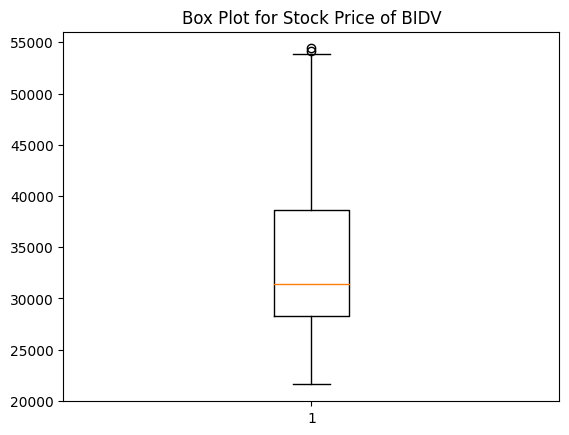
\includegraphics[width=1\textwidth]{resources/chapter-3/newdata/Boxplot_BIDV.png}
    \caption{Biểu đồ boxplot của giá cổ phiếu BIDV}
    \label{fig:bidv_boxplot}
    \end{minipage}
    \hfill
    \begin{minipage}{0.23\textwidth}
    \centering
    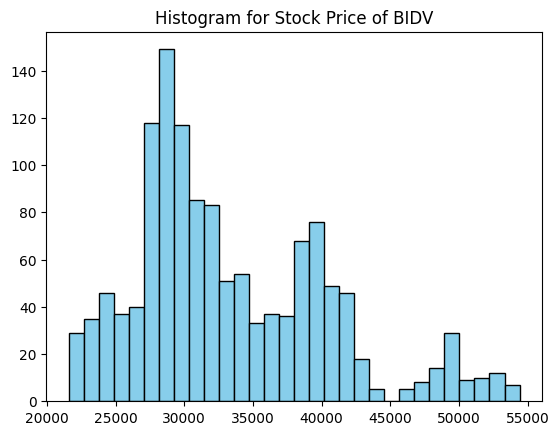
\includegraphics[width=1\textwidth]{resources/chapter-3/newdata/Histogram_BIDV.png}
    \caption{Biểu đồ histogram của giá cổ phiếu BIDV}
    \label{fig:bidv_histogram}
    \end{minipage}
\end{figure}

\begin{figure}[H]
    \centering
    \begin{minipage}{0.23\textwidth}
    \centering
    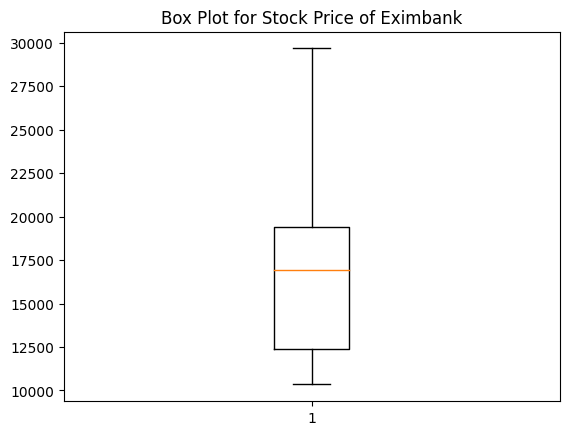
\includegraphics[width=1\textwidth]{resources/chapter-3/newdata/Boxplot_Eximbank.png}
    \caption{Biểu đồ boxplot của giá cổ phiếu Eximbank}
    \label{fig:eximbank_boxplot}
    \end{minipage}
    \hfill
    \begin{minipage}{0.23\textwidth}
    \centering
    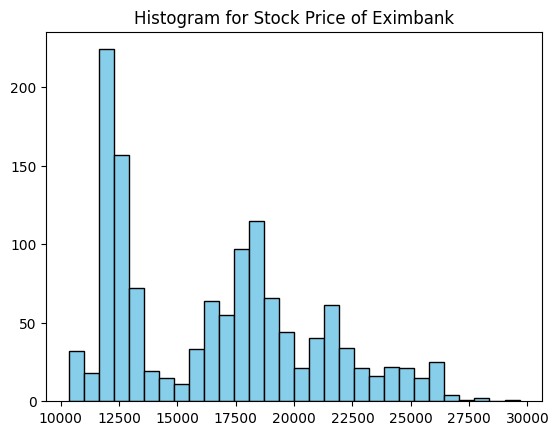
\includegraphics[width=1\textwidth]{resources/chapter-3/newdata/Histogram_Eximbank.png}
    \caption{Biểu đồ histogram của giá cổ phiếu Eximbank}
    \label{fig:eximbank_histogram}
    \end{minipage}
\end{figure}

\begin{figure}[H]
    \centering
    \begin{minipage}{0.23\textwidth}
    \centering
    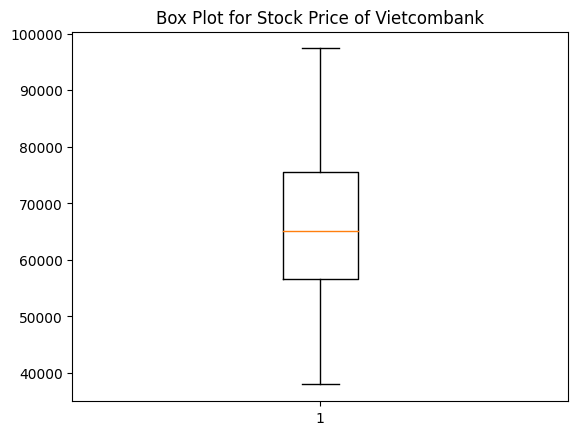
\includegraphics[width=1\textwidth]{resources/chapter-3/newdata/Boxplot_Vietcombank.png}
    \caption{Biểu đồ boxplot của giá cổ phiếu Vietcombank}
    \label{fig:vcb_boxplot}
    \end{minipage}
    \hfill
    \begin{minipage}{0.23\textwidth}
    \centering
    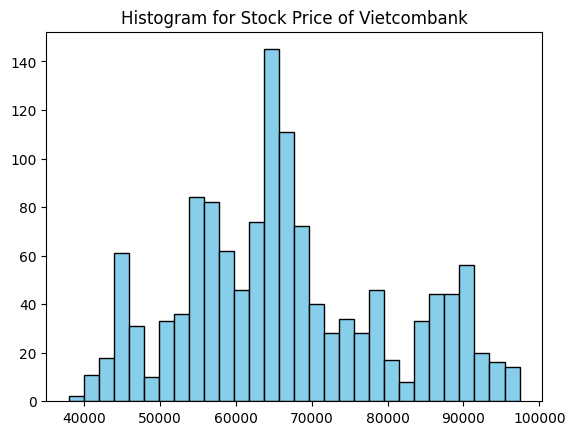
\includegraphics[width=1\textwidth]{resources/chapter-3/newdata/Histogram_Vietcombank.png}
    \caption{Biểu đồ histogram của giá cổ phiếu Vietcombank}
    \label{fig:vcb_histogram}
    \end{minipage}
\end{figure}

\subsection{Công cụ}
Trong nghiên cứu này, chúng em đã sử dụng các công cụ phân tích thống kê khác nhau trong Python bao gồm numpy, pandas, sklearn và matplotlib.pyplot.
% end hoang

\subsection{Tỷ lệ phân chia tập dữ liệu}
Phân chia dữ liệu thành hai tập: tập train và tập test theo các tỷ lệ 7:3, 8:2, 9:1. Tỷ lệ tiêu chuẩn là 7:3, tức là sử dụng 70\% dữ liệu cho việc train và 30\% cho việc test. Tỷ lệ này thường được sử dụng bởi vì với một bộ dữ liệu lớn và cần đạt được độ chính xác cao trong đánh giá mô hình. Bên cạnh đó, tỷ lệ 8:2 được coi là tỷ lệ tốt nhất cho việc phân chia tập train và tập test. Tỷ lệ này thường được sử dụng khi bộ dữ liệu có kích thước lớn và sẽ giúp mô hình được train với nhiều thông tin hơn từ dữ liệu. Cuối cùng, tỷ lệ 9:1 có train gần với test sẽ giúp mô hình học được nhiều thông tin hơn từ tập huấn luyện và đánh giá hiệu quả tốt trên tập kiểm tra.

\subsection{Các chỉ số đánh giá mô hình}
Để đánh giá độ chính xác của các mô hình, sử dụng ba tham số là Mean Absolute Error (MAE), Mean Absolute Percentage Error (MAPE) và Root Mean Squared Error (RMSE). Các giá trị này càng nhỏ thì mô hình càng tốt.
\par
\textbf{RMSE} được tính bằng cách lấy căn bậc hai của trung bình bình phương sai số giữa các giá trị dự đoán và các giá trị thực tế.
\[
\text{RMSE} = \sqrt{\frac{1}{n} \sum_{i=1}^{n} (y_i - \hat{y}_i)^2}
\]
\par
\textbf{MAPE} còn được gọi là độ lệch phần trăm tuyệt đối trung bình. Nó thường biểu thị độ chính xác dưới dạng tỷ lệ được xác định bởi công thức:
\[
\text{MAPE} = \frac{1}{n} \sum_{i=1}^{n} \left| \frac{y_i - \hat{y}_i}{y_i} \right| \times 100
\]
\par
\textbf{MAE} được đo bằng cách tính trung bình giá trị tuyệt đối của sai số giữa giá trị thực tế và giá trị dự đoán.
\[
\text{MAE} = \frac{1}{n} \sum_{i=1}^{n} |y_i - \hat{y}_i|
\]